\section{Results}

\subsection{Folded Manifold Reconstruction}

Figure~\ref{fig:manifold} addresses the first question in the evidence chain: whether campaigns with distinct forcing and measurement geometry still recover a common folded topology in reduced coordinates. Across CASES-99, FLOSS, GABLS3, and BLLAST, the reconstructed trajectories populate branch-separated regions in $(\eta_1,\eta_2,\eta_3)$ that are consistent with folded-sheet organization. The direct observation is geometric: campaign-specific offsets exist, but fold-like branch structure and transition corridors remain visible in each case.

This figure is intentionally descriptive rather than mechanistic. It establishes cross-campaign topological persistence before any claims about transition timing or trigger order. The interpretive boundary is explicit: we infer structural compatibility with equilibrium-fold dynamics, not proof of a unique canonical catastrophe model.

This first panel anchors the remainder of Results. Figure~\ref{fig:archetypes} then tests whether differences in observed transition character can be represented as campaign-dependent fold-edge geometry within the same shared manifold framework.

\begin{figure}[t]
	\centering
	\includegraphics[width=\columnwidth]{figures/fig4_manifold.pdf}
	\caption{\label{fig:manifold}Campaign manifold reconstruction in reduced coordinates $(\eta_1,\eta_2,\eta_3)$ showing branch-separated folded-sheet geometry across CASES-99, FLOSS, GABLS3, and BLLAST. The plotted structure is a direct geometric observation from campaign-wise p-FEM reconstruction; interpretation is limited to topological compatibility with equilibrium-fold organization.}
\end{figure}

% DRAFTING NOTE:
% Establish the shared topological claim first: all campaigns project to a folded
% sheet with branch-separated transition corridors, even when forcing context differs.

\subsection{Brittle Versus Rubbery Transition Archetypes}

Figure~\ref{fig:archetypes} asks whether campaign-to-campaign differences in transition character map to differences in local fold-edge sharpness rather than to different governing physics. CASES-99 exhibits a steeper fold-adjacent departure behavior (brittle archetype), while FLOSS exhibits a shallower fold-proximal passage with longer residence near marginal stability (rubbery archetype). The observational claim is that these contrasting trajectory patterns are both representable in the same folded coordinate chart.

Interpretively, this panel reframes campaign contrast as variation in geometric transversality within a shared structural class. Causal language remains bounded: we report observed associations between fold-proximal trajectory shape and transition character, while reserving universal trigger claims for campaign-complete verification.

With archetype structure established, Figure~\ref{fig:shadow} turns to the projection problem directly by comparing local Richardson diagnostics with non-local curvature-mode evolution through transition intervals.

\begin{figure}[t]
	\centering
	\includegraphics[width=\columnwidth]{figures/fig5_archetypes.pdf}
	\caption{\label{fig:archetypes}Transition archetypes contrasting brittle and rubbery fold behavior across campaign contexts. CASES-99 and FLOSS illustrate distinct fold-proximal trajectory classes within the same manifold family, consistent with differences in local transversality while preserving shared folded topology.}
\end{figure}

% DRAFTING NOTE:
% Tie terrain-dependent structure directly to observed transition character.
% Keep wording observational where causal ordering is not directly measured.

\subsection{Projection Shadows in Time Series}

Figure~\ref{fig:shadow} evaluates the chart-equivalence claim in time-domain diagnostics. The central observation is that local $\Rig$ can saturate in supercritical intervals while $\eta_3$ continues to evolve, preserving sensitivity to ongoing column-scale deformation. This is the expected signature of projection compression: distinct manifold states can map to similar local-gradient values when trajectories run near fold direction.

The evidentiary emphasis is operational, not rhetorical. We compare temporally aligned diagnostics and report where non-local curvature evolution remains informative after local-threshold metrics flatten. This supports the embedding interpretation of Richardson diagnostics as local indicators inside a broader state-surface evolution.

Figure~\ref{fig:slowing} extends this comparison by quantifying fold-proximal precursor behavior using lag structure and slowing-down diagnostics.

\begin{figure}[t]
	\centering
	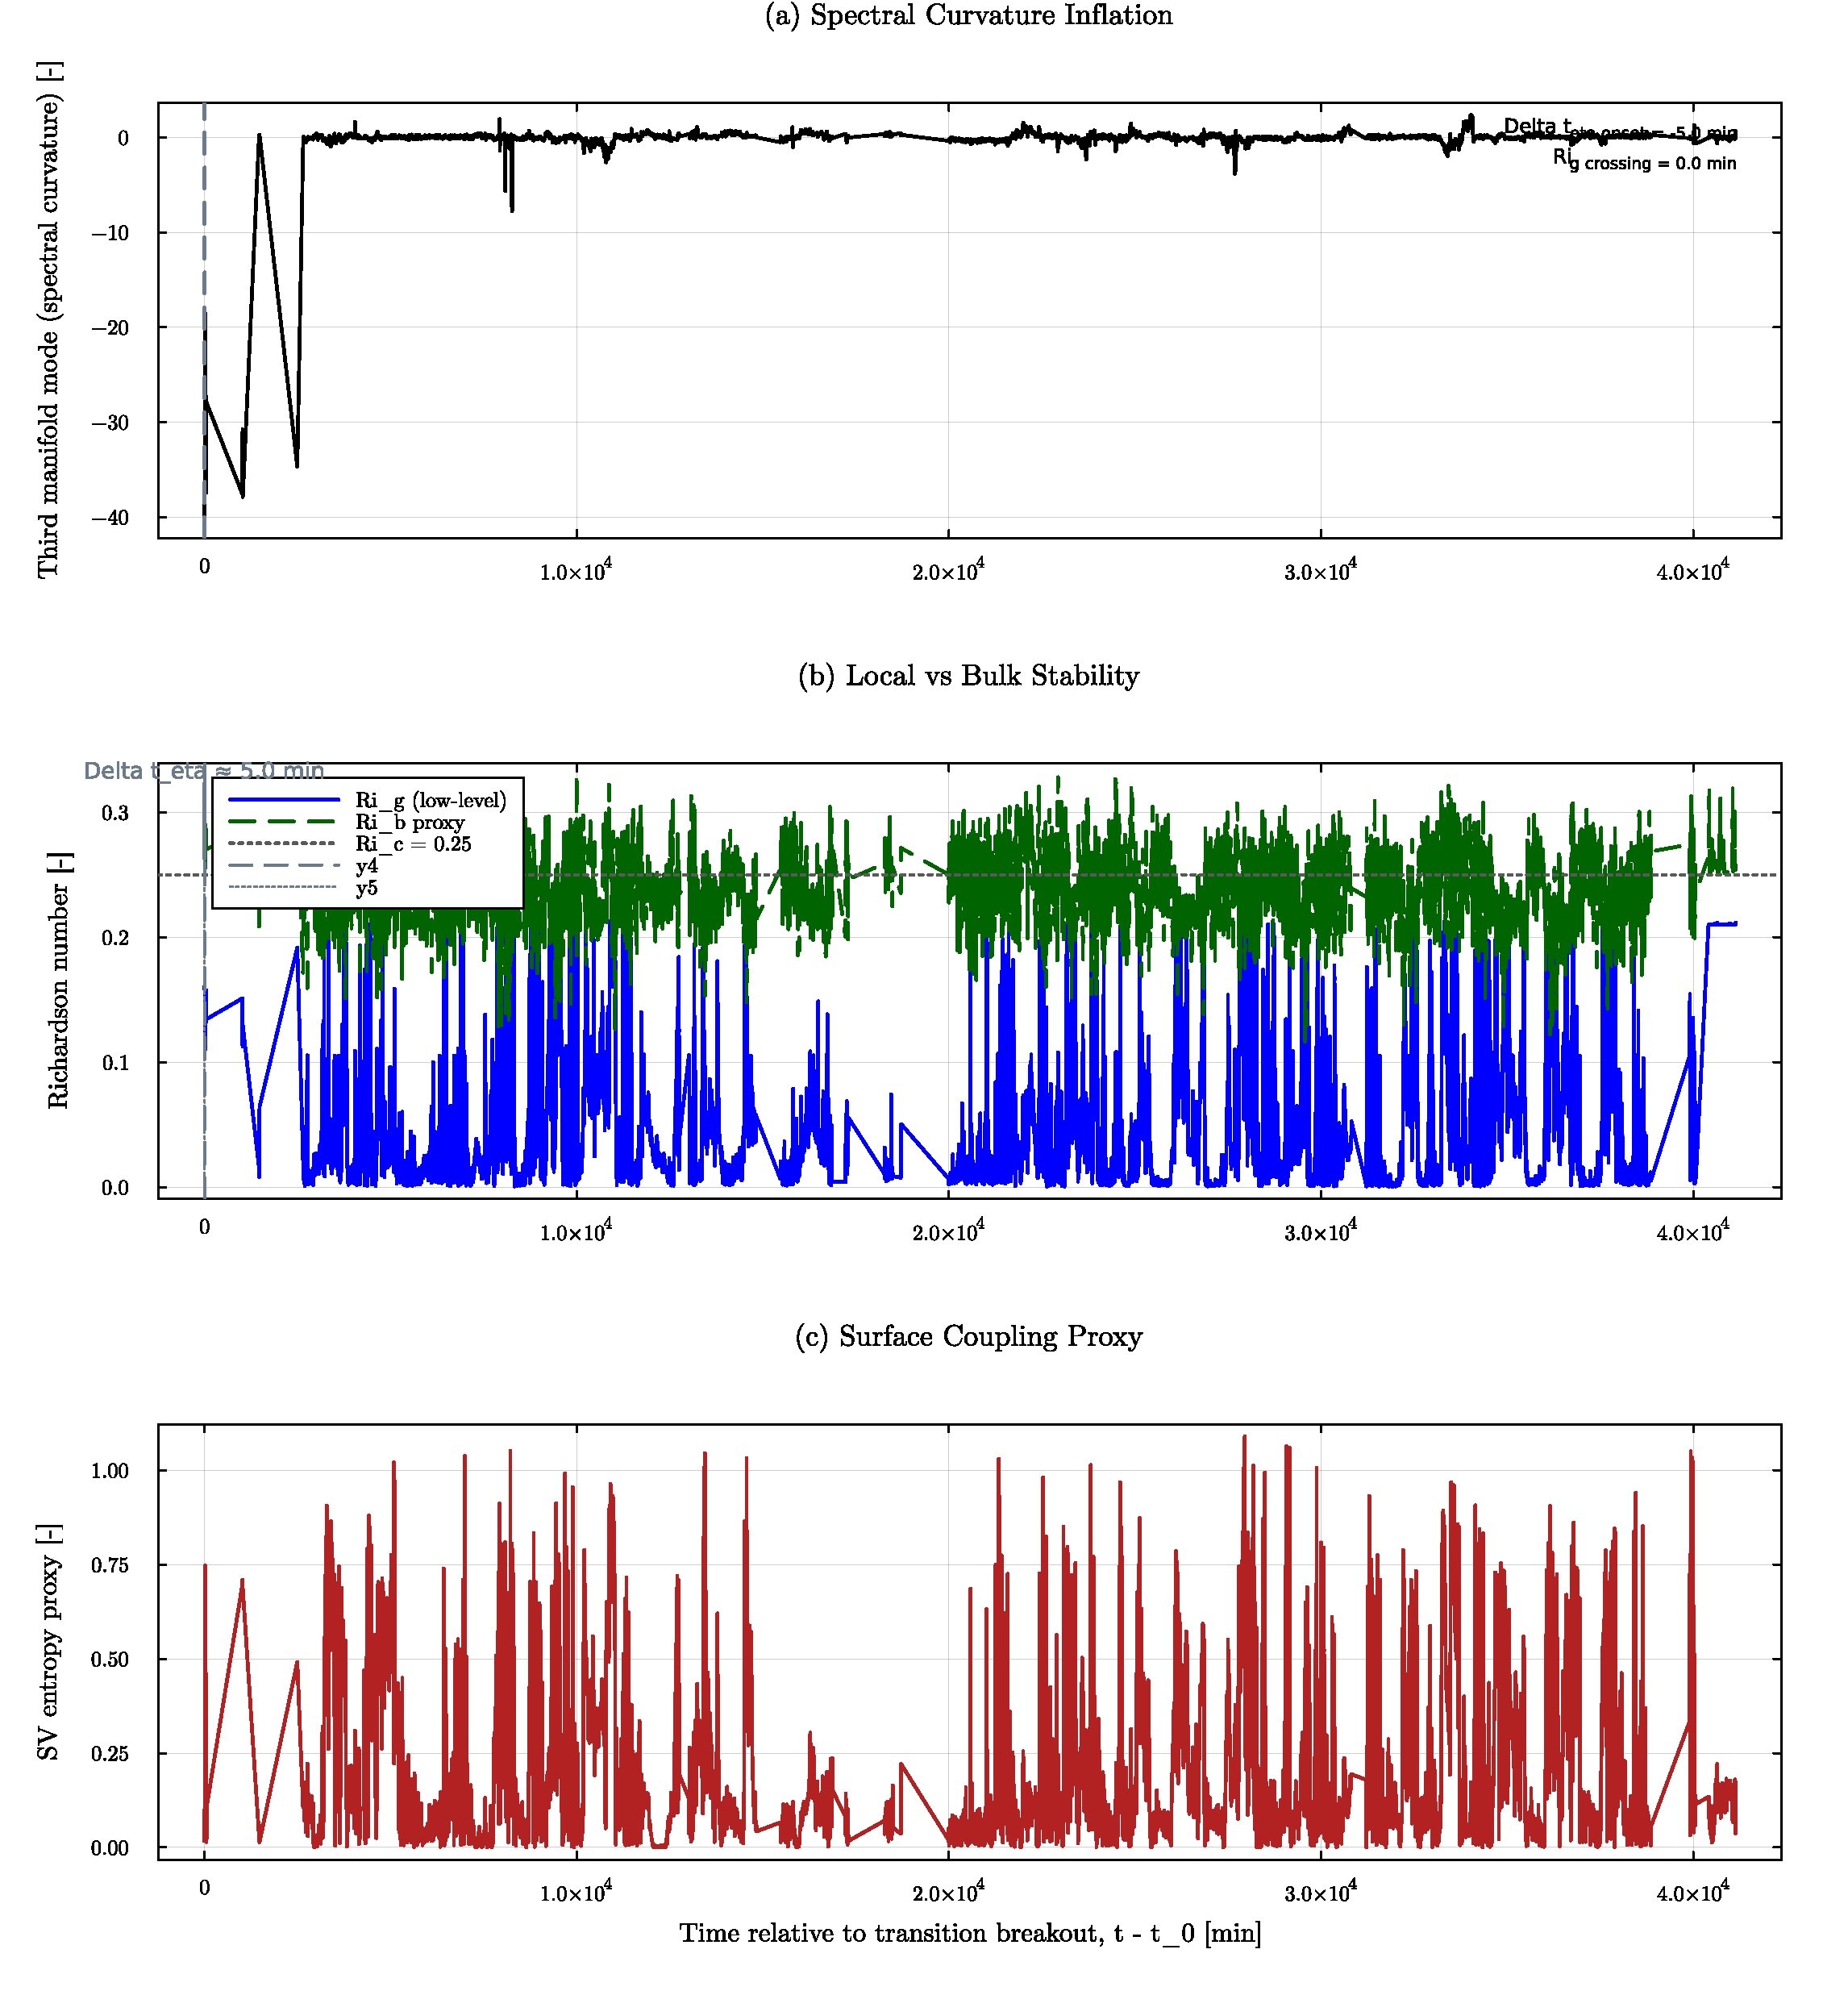
\includegraphics[width=\columnwidth]{figures/fig6_shadow_timeseries.pdf}
	\caption{\label{fig:shadow}Time-series projection shadowing: local Richardson diagnostics versus non-local manifold curvature mode evolution. Intervals where $\Rig$ is weakly varying but $\eta_3$ continues to change are interpreted as projection-compressed states, consistent with fold-proximal motion in the reduced chart.}
\end{figure}

% DRAFTING NOTE:
% Explicitly state where Ri_g saturates while eta_3 remains informative.
% This section is where projection singularity language should anchor to data.

\subsection{Critical Slowing and Precursor Geometry}

Figure~\ref{fig:slowing} asks whether approach to fold-proximal neighborhoods is accompanied by measurable precursor structure in campaign diagnostics. The direct measurements are lag-correlation organization and reduced-coordinate precursor behavior near transition-prone segments. Where available, these diagnostics are paired with campaign-scoped mutual-information summaries to quantify dependence in subcritical intervals.

Interpretation remains constrained to observed ordering and association in each dataset. We do not claim a universal causal sequence across all forcing regimes in this panel alone; rather, we document reproducible precursor signatures that are consistent with geometric approach-to-fold dynamics.

Figure~\ref{fig:collapse} then tests portability by examining whether curvature-mode behavior admits a campaign-agnostic collapse against fold-distance coordinates.

\begin{figure}[t]
	\centering
	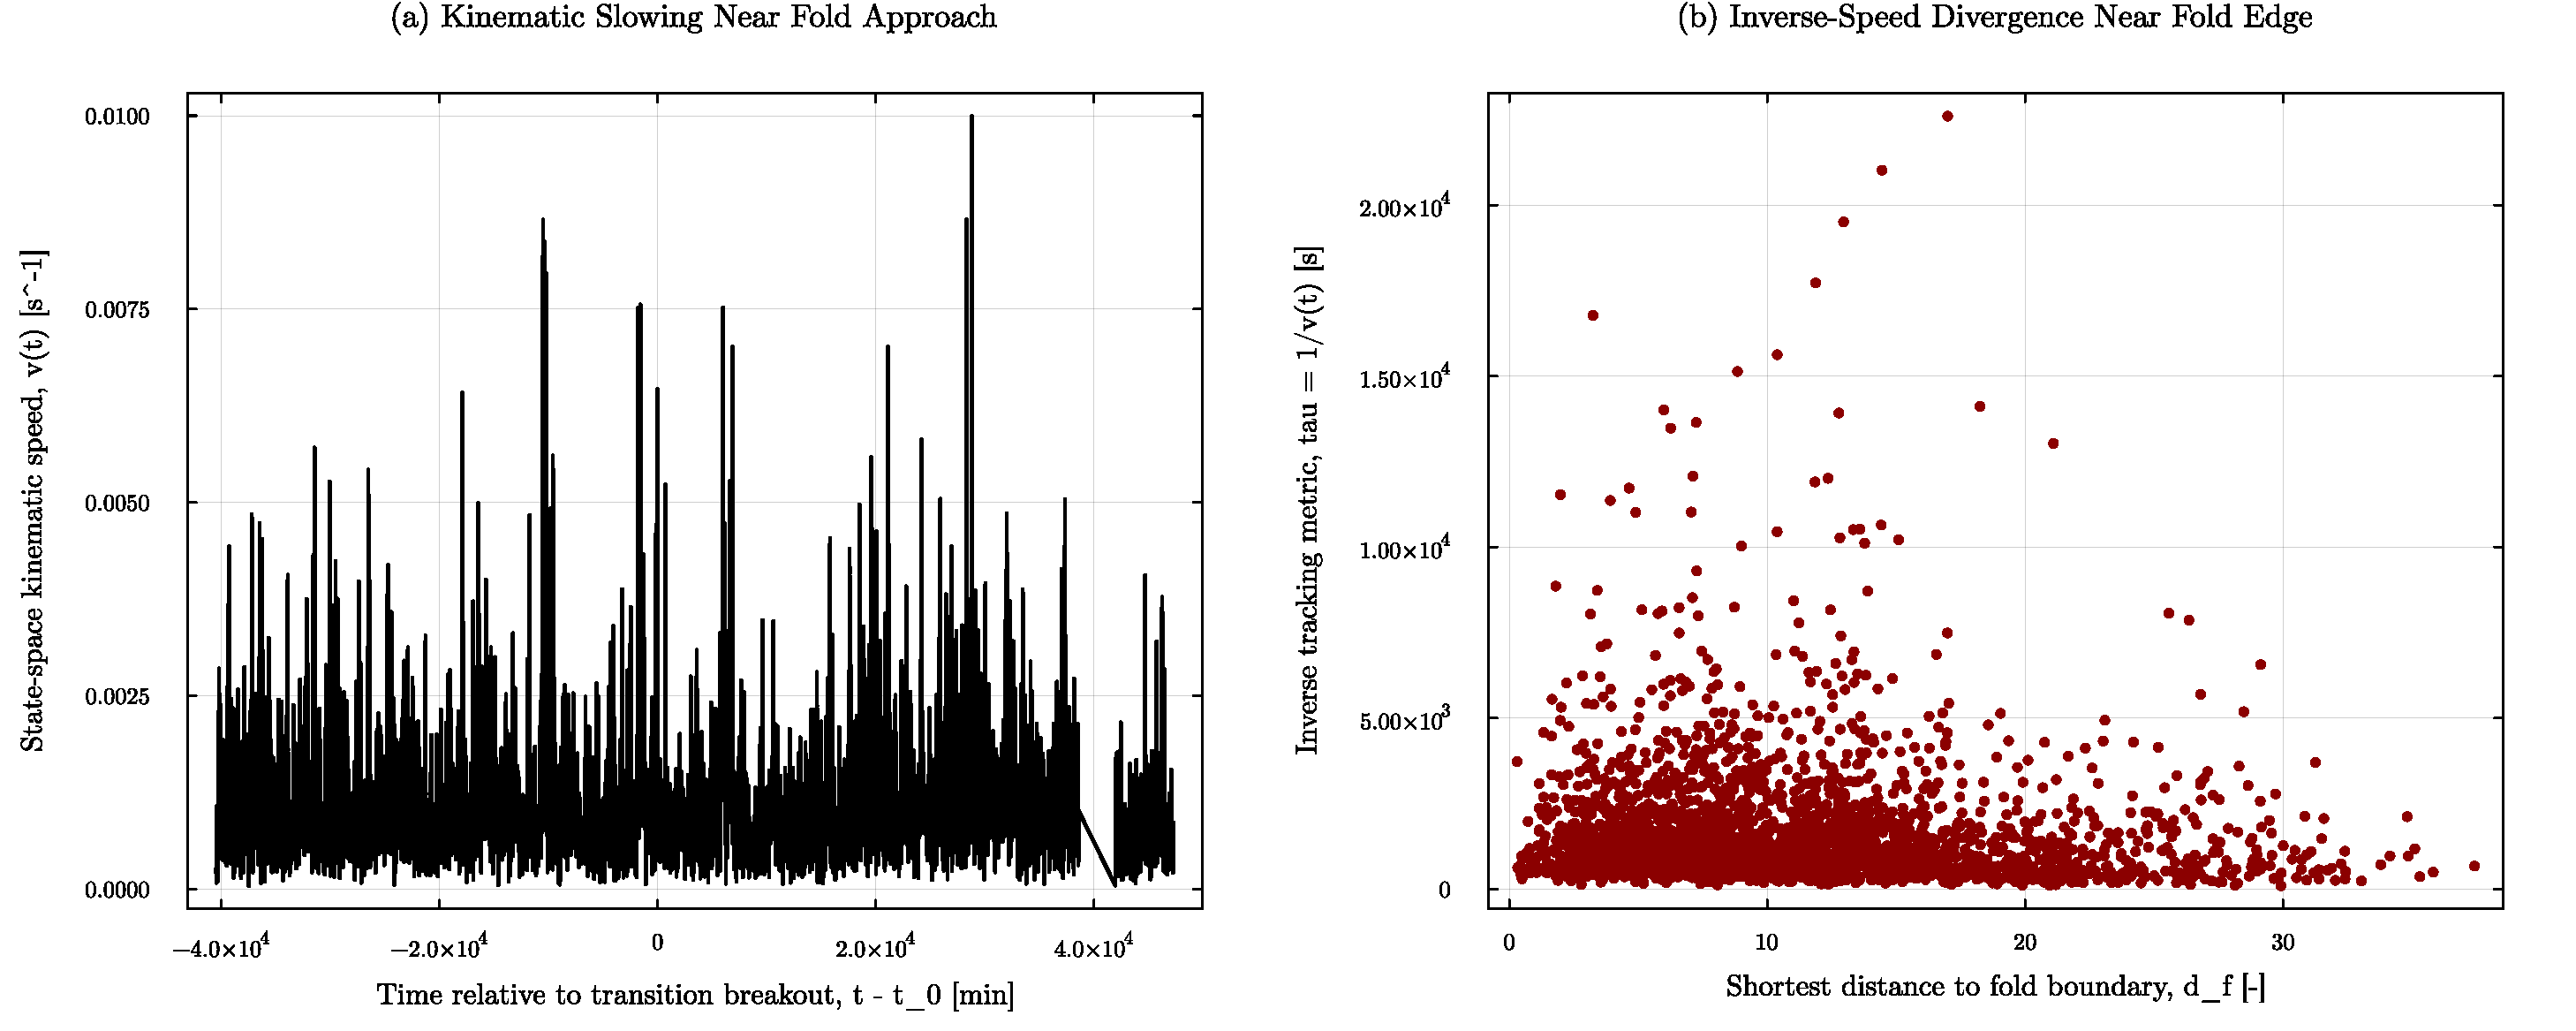
\includegraphics[width=\columnwidth]{figures/fig7_slowing_down.pdf}
	\caption{\label{fig:slowing}Critical-slowing diagnostics and precursor geometry near fold-proximal states. Reported lag and dependence patterns are campaign-scoped observations used as geometric early-warning evidence, not standalone proof of cross-campaign causal universality.}
\end{figure}

% DRAFTING NOTE:
% Cross-reference lag and mutual-information metrics exported by generated macros.

\subsection{Universal Collapse in Curvature Coordinates}

Figure~\ref{fig:collapse} is the portability test for the figure sequence. The question is whether campaign-resolved $\eta_3$ behavior can be represented in a shared scaling relation against distance-to-fold coordinates without erasing known contextual differences. The observational claim is the presence of a compact collapse trend in reduced geometric space across selected campaign/model pairs.

The interpretation is deliberately bounded. A successful collapse supports geometric transferability of the curvature coordinate framework; it does not imply that all transition pathways, forcing mechanisms, or timescales are identical across campaigns. This distinction preserves compatibility with both field heterogeneity and LES idealization limits.

\begin{figure}[t]
	\centering
	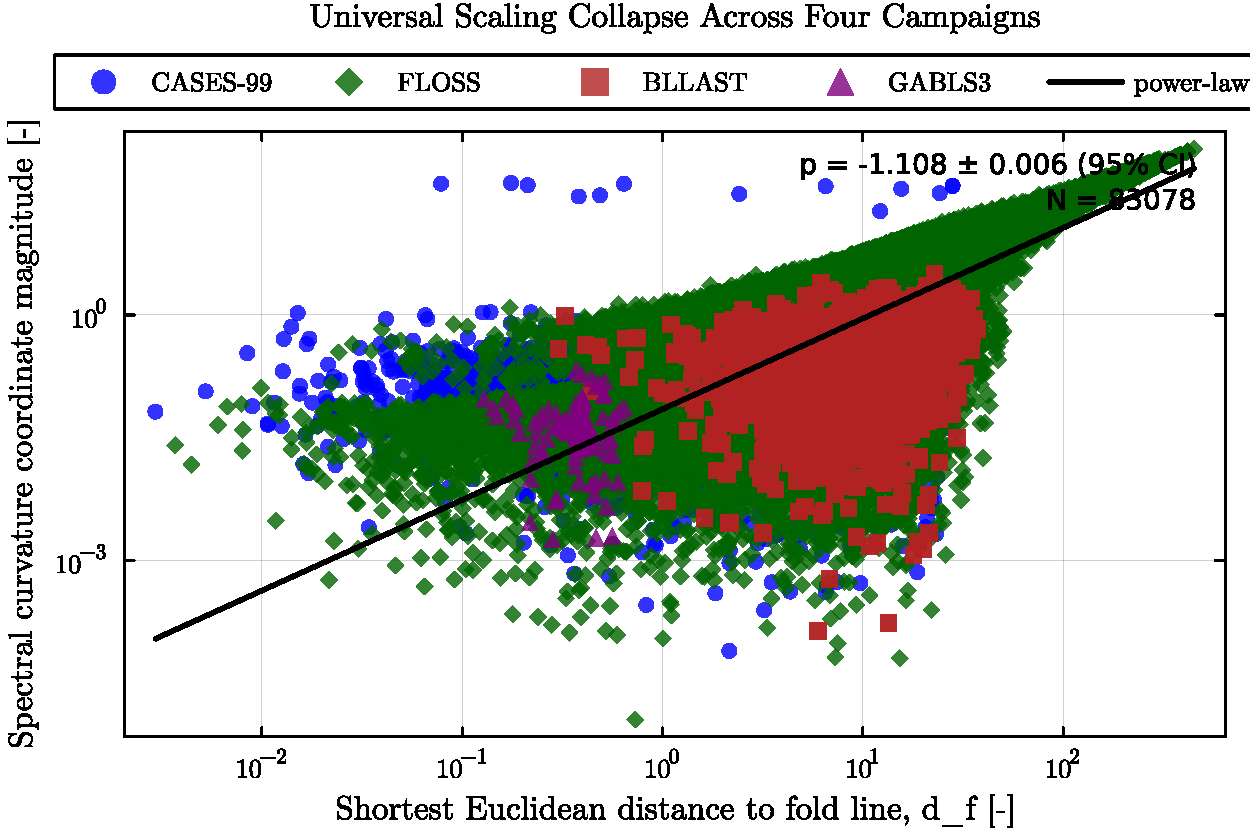
\includegraphics[width=\columnwidth]{figures/fig8_universal_collapse.pdf}
	\caption{\label{fig:collapse}Universal-collapse test of the third manifold mode ($\eta_3$) as a function of shortest Euclidean distance to the fold line ($d_f$). The collapse is interpreted as evidence of transferable geometric organization in reduced coordinates, with causal and dynamical claims restricted to directly measured campaign/model diagnostics.}
\end{figure}

% DRAFTING NOTE:
% The data collapse across CASES-99 and GABLS3 is the central portability claim.
% Keep this section tightly coupled to pipeline-generated fit diagnostics.
